\section{Deep Generative Models}
\begin{itemize}
	\item \textit{Generative modeling}: learn the joint probability $p(x,y)$ or density function $p(x)$. Task can be performed with Bayes rule: $p(y|x)$. Generalize better (less prone to overfitting), and better modeling of causal relations. Members include GAN, VAE, etc.
	\begin{itemize}
		\item We can use generative models to predict uncertainty and out of distribution examples: $p(x,y) = p(y|x)p(x) \Rightarrow$ if $x$ o.o.d., then $p(x)$ low!
	\end{itemize}
	\item \textit{Discriminative modeling}: learn conditional pdf $p(y|x)$. Is usually task-oriented and gets better results. 
	\item Applications of generative models
	\begin{itemize}
		\item Simulating possible futures for reinforcement learning
		\item Creating missing data  (e.g. pixel patches which are missing)
		\item Super-resolution scaling for images
		\item Data augmentation (replace e.g. car by bicyclist in a scene)
		\item Cross-modal translation (sketch to image)
	\end{itemize}
	\item Different type of generative models (see Figure~\ref{fig:GAN_generative_models_overview})
	\begin{itemize}
		\item \textit{Explicit density}: maximize log likelihood of the data by modeling a probability density function. Function must be complex enough and computationally tractable
		\item \textit{Implicit density}: no explicit pdf needed, only a sampling mechanism
	\end{itemize}
	\begin{figure}[ht!]
		\centering
		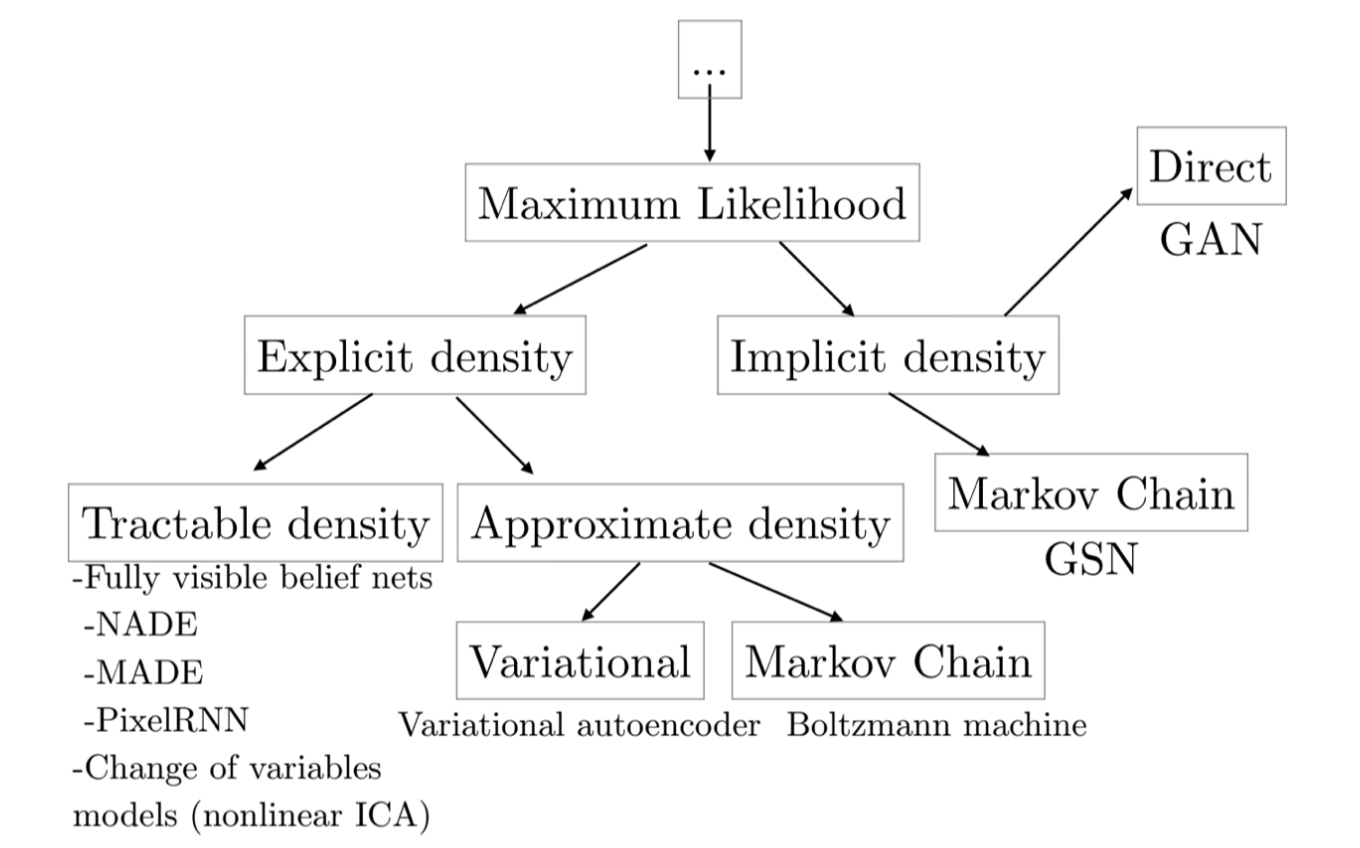
\includegraphics[width=0.45\textwidth]{figures/GAN_generative_models_overview_2.png}
		\caption{Overview of generative models}
		\label{fig:GAN_generative_models_overview}
	\end{figure}
\end{itemize}
\subsection{Generative Adversarial Networks}
\begin{itemize}
	\item Adversarial training of generator vs discriminator
	\begin{figure}[ht!]
		\centering
		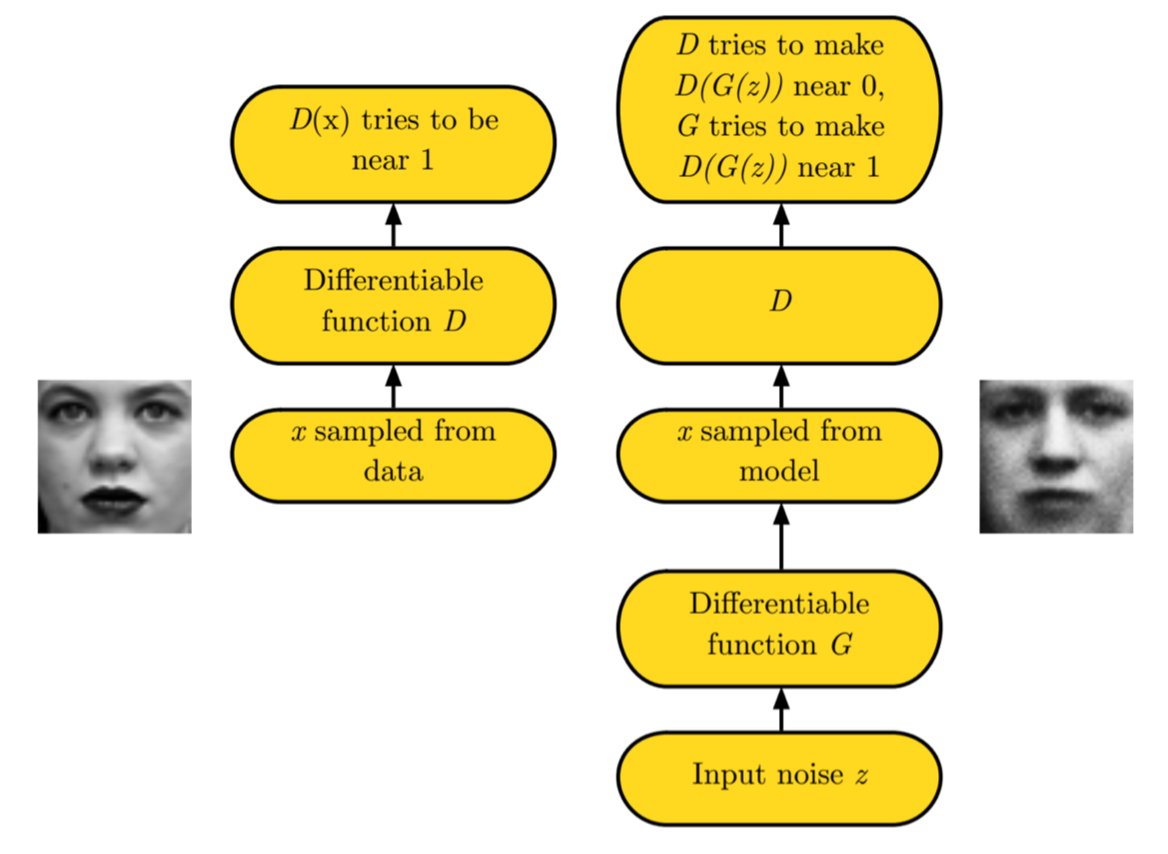
\includegraphics[width=0.45\textwidth]{figures/GAN_pipeline.png}
		\caption{Pipeline of adversarial GAN training}
		\label{fig:GAN_pipeline}
	\end{figure}
	\item The generator is a (mostly deconvolutional) network that takes noise $z$ as input, and creates fake images. The discriminator tries to distinguish between fake and real images
	\item Trained in a minimax game fashion, the loss function resembles the Jensen-Shannon divergence:
	\begin{equation*}
		\begin{split}
			\min_G \max_D V(G,D) & = \mathbb{E}_{\bm{x}\sim p_{\text{data}}(\bm{x})} \left[\log \left(D\left(\bm{x}\right)\right)\right] + \mathbb{E}_{\bm{z}\sim p_{z}(\bm{z})} \left[\log\left(1 - D\left(G\left(\bm{z}\right)\right)\right)\right] \\
			J^{(D)} & = - \frac{1}{2}\mathbb{E}_{x\sim p_{\text{data}}}\left[\log D(x)\right] - \frac{1}{2}\mathbb{E}_{z\sim p_{z}}\left[\log 1 - D(G(z))\right]\\
			J^{(G)} & = - \frac{1}{2}\mathbb{E}_{z\sim p_{z}}\left[\log D(G(z))\right]\\
		\end{split}
	\end{equation*}
	\item Loss of generator is changed from $\log 1 - D(G(z))$ because otherwise the gradients of the generator vanish for a too strong discriminator 
	\item Divergence is important and can strongly influence the behavior of model
	\begin{equation*}
		\begin{split}
			D_{KL}\left(p(x)\lVert q^{*}(x)\right) = \int p(x) \log \frac{p(x)}{q^{*}(x)} dx & \implies \text{if } p(x)>0, \text{ then } q(x)>0\\
			D_{KL}\left(q^{*}(x)\lVert p(x)\right) = \int q^{*}(x) \log \frac{q^{*}(x)}{p(x)} dx & \implies \text{if } p(x)=0, \text{ then } q(x)=0\\
		\end{split}
	\end{equation*}
\end{itemize}
\subsubsection{GAN training problems}
\begin{itemize}
	\item \textbf{Vanishing gradients} during training:
	\begin{itemize}
		\item If the discriminator is too bad, the generator does not get valid/accurate feedback and can therefore not learn properly
		\item If the discriminator is perfect, the generator has very low gradients as a small change does not influence the discriminator
		\begin{figure}[ht!]
			\centering
			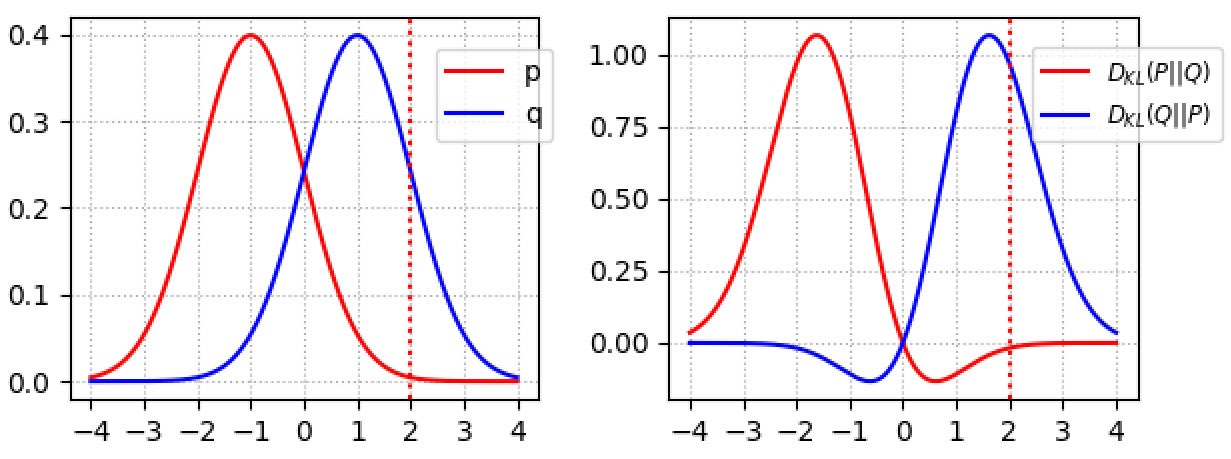
\includegraphics[width=0.4\textwidth]{figures/cv_deep_learning_GAN_vanishing_gradients.jpeg}
			\caption{Vanishing gradients problem for training with KL-divergence. When the distance between the two distributions $p$ and $q$ (respectively $P_g$ and $P_r$) is too huge, the KL divergence is very close to zero. Hence, is does not provide any strong gradients in these regions.}
		\end{figure}
	\end{itemize}
	\item \textbf{Reaching the equilibrium}
	\begin{itemize}
		\item We know that the nash equilibrium of the minimax game is $P_g=P_r$ meaning the distribution of the real data is equal to the generated data. In that case, $D$ return 0.5 no matter what example we put in (as both distributions are equal).
		\item However, it has been shown that such cost functions may not converge when using gradient descent. An example is shown in Figure~\ref{fig:GAN_reaching_equilibrium}.
		\begin{figure}[ht!]
			\centering
			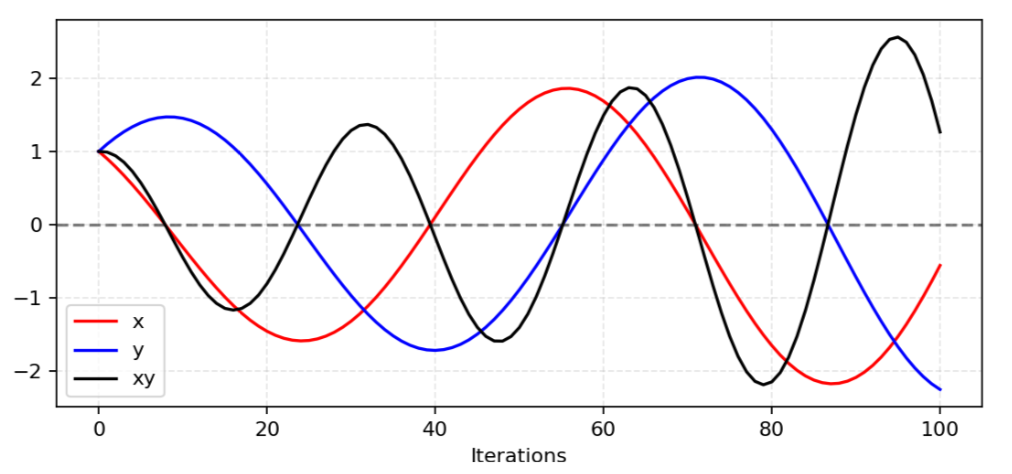
\includegraphics[width=0.4\textwidth]{figures/cv_deep_learning_GAN_oscillating.png}
			\caption{Oscillating behavior of a non-cooperative game where $\min_x \max_y V(x,y) = x\cdot y$. The equilibrium $x=y=0$ is never reached.}
			\label{fig:GAN_reaching_equilibrium}
		\end{figure}
	\end{itemize}
	\item \textbf{Mode collapse}
	\begin{itemize}
		\item A GAN suffers from a mode collapse if the generator limits its predictions/generated distribution to a few samples/modes.
		\item For example in case of the MNIST dataset, this would mean that the generator only creates numbers of one or two different digits. Although a full mode collapse is rarely the case, partial mode collapses frequently occur
		\item In order to create a mode collapse, the gradients regarding the noise $\bm{z}$ must be very low/close to zero. This can for example happen if we fix the discriminator and the generator converges to the optimal image $\bm{x}^*$ that fools the discriminator the most
		\item Once the generator collapse to one mode, the discriminator will learn that this mode is purely/mostly generated and thus changes its predictions. The generator will address that by changing the mode (note that as $\partial L/\partial \bm{z}\approx 0$, we will just collapse to the next mode and are not able to escape this loop).
		\item In the end, this turns into a cat-and-mouse game between the generator and discriminator, and will not converge (see Figure~\ref{fig:GAN_mode_collapse}).
		\begin{figure}[ht!]
			\centering
			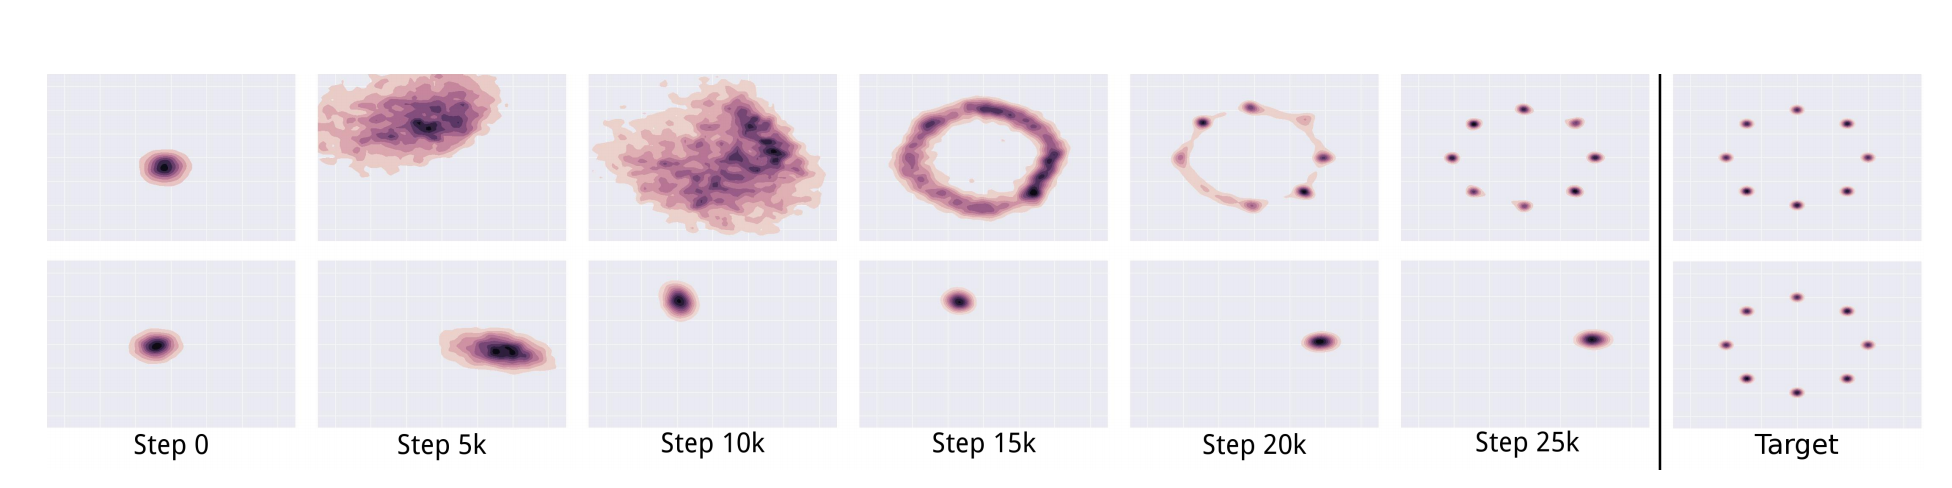
\includegraphics[width=0.6\textwidth]{figures/cv_deep_learning_GAN_mode_collapse.png}
			\caption{\textit{Top row}: optimal convergence of generator distribution to 8 modes. \textit{Bottom row}: Sample of a mode collapse after 10k iterations. The generator is only able to generate a single mode.}
			\label{fig:GAN_mode_collapse}
		\end{figure}
	\end{itemize}
	\item \textbf{Low dimensional support}
	\begin{itemize}
		\item The KL and JS divergence work best for overlapping distributions as neither of them is 0 (numerical instability)
		\item However, during training, the training distribution is not perfect, and as we have high dimensional data, both distributions are less likely to overlap much
		\item Also, it is easy for the discriminator to find a line in between them
	\end{itemize}
\end{itemize}
\subsubsection{GAN improvements}
\begin{itemize}
	\item \textbf{Wasserstein GAN}
	\begin{itemize}
		\item Instead of KL/JS, use Wasserstein (Earth Mover's) Distance:
		$$\mathcal{W}(p_r, p_g) = \inf\limits_{\gamma \sim \prod (p_r,p_g)} \mathbb{E}_{(x,y)\sim \gamma}|x-y|$$
		\item Intuitive explanation: how much do I have to move from one distribution to get the other one. Thus, the distance is even meaningful for non-overlapping distributions
	\end{itemize}
	\item \textbf{Usage of labels}
	\begin{itemize}
		\item Learning a conditional model $p(y|x)$ often generates better samples than from a random distribution
		\item One example are conditional GANs where we have given a ground truth
	\end{itemize}
	\item \textbf{Label smoothing}
	\begin{itemize}
		\item Train the discriminator to predict $D(x)\approx 1 - \alpha$ instead of 1
		\item Has been shown to be a good regularization by preventing the discriminator to be overconfident
		\item In addition, the gradients of the generator do less likely explode
	\end{itemize}
	\item \textbf{Virtual batch normalization}
	\begin{itemize}
		\item Batch Normalization can significantly help in neural networks
		\item However, in GANs, it leads to high intra-batch correlation
		\item Solution: \textit{virtual batch normalization} where we select a reference batch which is fixed during training, and combine it with the statistics of the current batch. Reduces overfitting on reference batch and intra-batch correlation
	\end{itemize}
\end{itemize}
\subsubsection{GAN open questions}
\begin{itemize}
	\item \textbf{Mode collapse}: How to prevent a model to suffer from mode collapse. One idea is penalizing the model is features are too similar, or allowing discriminator to see across batch elements. But these solutions are more heuristic tries and no theoretical solution
	\item \textbf{Evaluation of GANs}: GANs are currently judged by their qualitative results/predictions, but there is no quantitative measurement yet
	\item \textbf{Discrete outputs}: The generator and discriminator need to be differentiable, and thus discrete outputs are not possible. There are some workarounds, but no real theoretically sound solution.
	\item \textbf{Semi-supervised classification}: How to combine a GAN training and discriminative model efficiently (discriminator predicts class and fake/real at the same time)
\end{itemize}
\subsection{Boltzmann machines}
\begin{itemize}
	\item A Boltzmann distribution is defined by $p(x) = \frac{1}{Z}\exp\left(-E\left(x\right)\right)$ where $E(x)$ is a energy function described by our model, and $Z=\sum\limits_x \exp\left(E\left(x\right)\right)$ a normalization constant
	\item The benefit of defining a distribution like that is that our model can use any output values between $[-\infty, \infty]$ instead of being constrained to $[0,1]$
	\item A problem is that even if $x$ is binary, the normalizing constant $Z$ gets out of hands (sum over $2^{n}$ combinations for $n$ dimensional $x$). Thus, we limit the computations by only considering pairwise relations
	\item Pairwise relations modeled by $E(x)=-x^TWx-b^Tx$. Learning $W$ and $b$ by maximizing the likelihood of the data
	\item Problem: $W$ is still of size $n^2$ which can be too large for e.g. images ($256\times 256$ leads to $4.2$ billion parameters in $W$) $\Rightarrow$ Restricted Boltzmann machines
\end{itemize}
\subsubsection{Restricted Boltzmann machines}
\begin{itemize}
	\item Restrict model by additional bottleneck over $h$ latents
	$$E(x,h) = -x^T W h - b^T x - c^T h, \hspace{2mm} p(x) = \frac{1}{Z}\sum_h \exp\left(-E\left(x,h\right)\right)$$
	\item This function is not in the form of a energy function anymore (because of the sum). We can rewrite it as:
	\begin{equation*}
		\begin{split}
			F(x) & = -b^T x - \sum_i \log \sum_{h_i} \exp\left(h_i\left(c_i + W_i x\right)\right)\\
			p(x) & = \frac{1}{Z} \exp\left(-F(x)\right)\\
			Z & = \sum\limits_x \exp\left(-F(x)\right)
		\end{split}
	\end{equation*}
	\item Can be represented as a single MLP layer (undirected) with less hidden units
	\item Compared to simple Boltzmann machine, we can express higher-order relations 
	\item Every hidden unit is independent of each other, and the same for input $x$:
	$$p(h|x) = \prod_j p(h_j|x, \theta), \hspace{2mm} p(x|h) = \prod_i p(x_i|h, \theta) $$
	\item We can now reformulate the conditional probabilities as sigmoids \textbf{iff} $h$ and $x$ are still binary:
	$$p(h_j|x, \theta) = \sigma\left(W_{:,j} x + b_j\right), \hspace{2mm}p(x_i|h, \theta) = \sigma\left(W_{i,:} h + c_i\right)$$
	\item The loss is maximizing the log likelihood:
	$$\mathcal{L}(\theta) = \frac{1}{N}\sum_n \log p(x_n|\theta) = \frac{1}{N}\sum_n\left[- F(x) - \log Z\right]$$
	\item The gradients can be computed accordingly:
	\begin{equation*}
		\begin{split}
			\pd{\log p(x_n|\theta)}{\theta} & = -\sum_h p(h|x_n, \theta) \pd{E(x_n,h| \theta)}{\theta} + \sum_{\tilde{x}, h} p(\tilde{x}, h|\theta) \pd{E(\tilde{x}, h|\theta)}{\theta}\\
		\end{split}
	\end{equation*}
	Problem: second term is sum over $x$ and $h$ $\Rightarrow$ high-dimensional, hard to compute
	\item One way to do it is using contrastive divergence: sample $h_0 \sim p(h|x)$, and $x_1 \sim p(x|h_0)$, etc. In practice, a single sample is mostly sufficient
	\item \textbf{Deep Belief Network}: RBM are still models of single layer, we can also use a stack of RBMs. First layer is directed, others not. Our joint pdf is $p(x, h_1, h_2) = p(x|h_1)\cdot p(h_1|h_2)$
	\item \textbf{Deep Boltzmann machines}: also a stack of RBMs, but with undirected first layer
	\begin{itemize}
		\item Hence, we get $p(h_2^{k}|h_1, h_3) = \sigma \left(W_1^{:,k}h_1 + W_3^{k,:}h_3 \right)$
		\item Computing gradients is intractable $\Rightarrow$ approximate by sampling
	\end{itemize}
\end{itemize}
\subsection{Variational Autoencoders}
\begin{itemize}
	\item We assume an underlying, lower-dimensional data distribution $p(z)$ with which we can model our data distribution $p(x,z)=p(x|z)p(z)$
	\item Therefore, we need to model $p(z|x)$ which is often not easy to compute. In variational inference, we approximate the true posterior by $q_{\varphi}(z)$ (approximated posterior does not have to depend on observed $x$, e.g. in VAE it does)
	\item Our goal is to maximize $p(x)$. As this is intractable, we use the ELBO:
	\begin{equation*}
		\begin{split}
			\log p(x) & = \log \int p(x,z)dz \\
			& = \log \int q_{\varphi}(z) \frac{\int p(x,z)}{q_{\phi}(z)} dz\\
			& = \log \mathbb{E}_{q_{\varphi}(z)}\left[\frac{p(x,z)}{q_{\varphi}(z)}\right]\\
			& \geq \mathbb{E}_{q_{\varphi}(z)}\left[\log \frac{p(x,z)}{q_{\varphi}(z)}\right]\\
			& = \mathbb{E}_{q_{\varphi}(z)}\left[\log p(x|z)\right] - \text{KL}\left(q_{\varphi}(z)||p(z)\right) = \text{ELBO}_{\theta, \varphi}\left(x\right)
		\end{split}
	\end{equation*}
	\item The distance between $\log p(x)$ and the ELBO is the KL divergence to the true (unknown) posterior:
	$$\log p(x) - \text{KL}\left(q_{\varphi}(z)||p(z|x)\right) = \mathbb{E}_{q_{\varphi}(z)}\left[\log p(x|z)\right] - \text{KL}\left(q_{\varphi}(z)||p(z)\right)$$
	\item Thus, maximizing the ELBO either increases the log likelihood or optimizes the approximated posterior
	\item Variational Autoencoders make $q_{\varphi}(z)$ dependent of $x$, and model $p_{\theta}(x|z)$ as well:
	$$\text{ELBO}_{\theta, \varphi}\left(x\right) = \mathbb{E}_{q_{\varphi}(z|x)}\left[\log p_{\theta}(x|z)\right] - \text{KL}\left(q_{\varphi}(z|x)||p_{\lambda}(z)\right)$$
	Note that $p_{\lambda}(z)$ is not optimized, and its parameters $\lambda$ just describe the prior (e.g. standard Gaussian) 
	\item The loss function for a VAE is the negative ELBO, where we approximate the expectation by a single sample. The KL is mostly chosen to be analytically solvable (e.g. for two Gaussian) to prevent a Monte-Carlo approximation of the integral 
	\item However, we face a problem when we try to compute the gradients for $\nabla_{\varphi} \mathcal{L}$. Using Monte-Carlo integration has high variance, and sampling is non-continuous operation
	\item \textbf{Reparameterization trick}: sample from external, constant distribution, and transform this sample into a sample of the modeled distribution. For Gaussian: $z = \mu_q + \sigma_q \cdot \epsilon$
\end{itemize}
\subsubsection{Improvements of VAE}
\begin{itemize}
	\item \textbf{Encoder distribution}
	\begin{itemize}
		\item Modeling $q(z|x)$ as Gaussian makes training and implementation easy, but assumes that true posterior is also Gaussian, or can be at least approximated by one
		\item Simple option: use different task-specific distribution like e.g. hyperspherical, however not always suitable
		\item We can improve the complexity of this posterior by plugging in a Normalizing flow on top of the encoder output
		\begin{equation*}
		\begin{split}
		z_0 \sim q_0(z|x) & = \mathcal{N}(z|\mu(x), \text{diag}(\sigma^2(x)))\\
		q_K(z|x) & = q_0(z|x) \cdot \left|\text{det}\pd{f_K(z_{k-1})}{z_{k-1}}\right|\\
		\end{split}
		\end{equation*}
		\item The ELBO is added with an additional term during training
		$$\text{ELBO} = \mathbb{E}_{q_{\varphi}(z|x)}\left[\log p_{\theta}(x|z)\right] - \text{KL}\left(q_{\varphi}(z|x)||p_{\lambda}(z)\right) + \mathbb{E}_{z_0 \sim q_0(z_0|x)}\left[\sum_{k=1}^{K} \log \left|\text{det}\pd{f_k(z_{k-1})}{z_{k-1}}\right|\right]$$
	\end{itemize}
	\item \textbf{Prior optimization}
	\begin{itemize}
		\item We assume a prior $p(z)$ which is for example Gaussian, but cannot make sure that every point of the prior actually has a realistic counterpart in the original $x$ space
		\item The optimal prior is the averaged distribution over all data samples: $q^{*}(z) = \frac{1}{N}\sum_{n=1}^{N} q_{\varphi}(z|x_n)$
		\item However, summing over all data point is infeasible. Thus, approximate it by $K$ pseudo-inputs $u_k$ that are trained via standard SGD in the framework:
		$$p_\lambda(z) = \frac{1}{K} \sum_{k=1}^{K} q_{\varphi}(z|u_k)$$
	\end{itemize}
	
\end{itemize}
\subsection{Normalizing flows}
\begin{itemize}
	\item VAE cannot model $p(x)$ directly because of the intractable formulation ($p(x) = \int p(x,z)dz$)
	\item Normalizing Flows solve that problem by using a series of invertible transformation that allow more complex latent distributions than Gaussian
	\item The models can therefore be trained on directly maximizing the log likelihood instead of using the ELBO or similar
	\item A normalizing flow consists of multiple flows that transform a simple Gaussian distribution step by step in the data distribution (see Figure~\ref{fig:NF_concept})
	\item Every flow shifts the probability mass specified by parameters (determined by e.g. a NN, see Figure~\ref{fig:NF_density_shift})
	\begin{figure}[ht!]
		% NF_density_shift.png
		\centering
		\begin{subfigure}{0.7\textwidth}
			\centering
			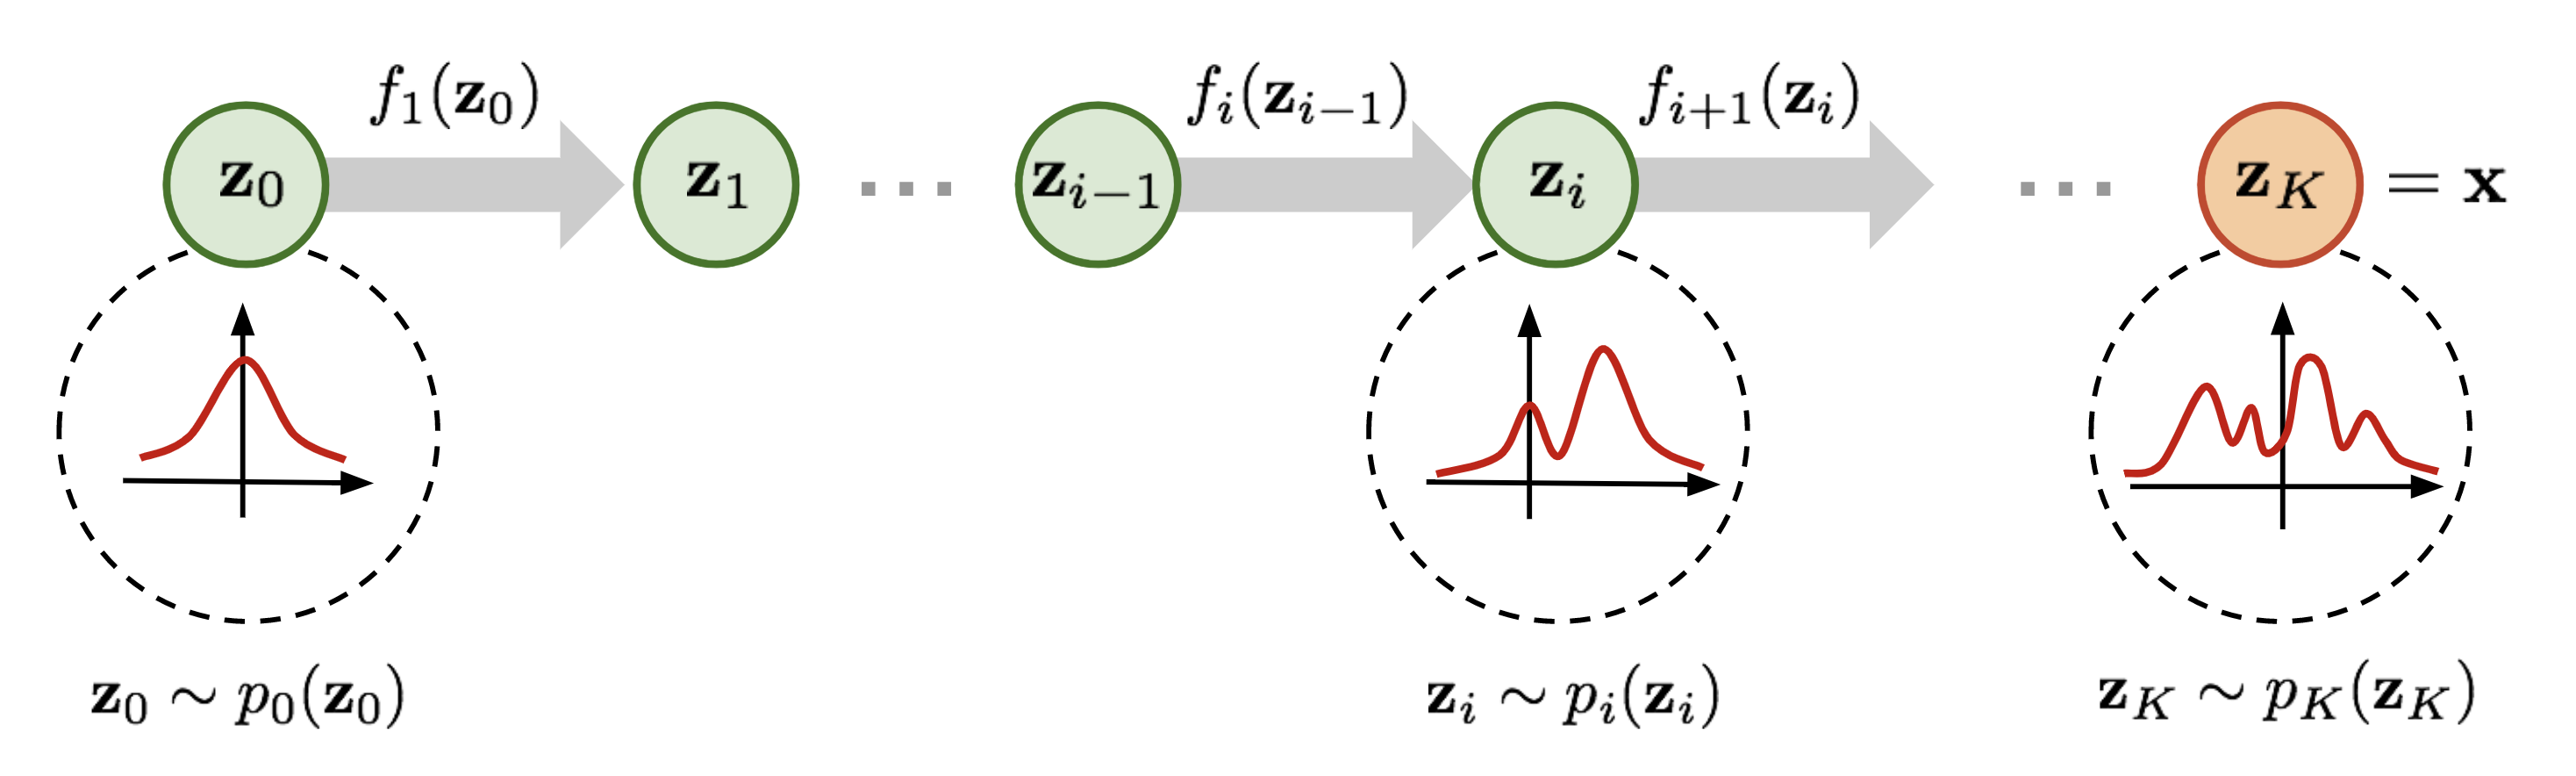
\includegraphics[width=\textwidth]{figures/NF_concept.png}
			\caption{General concept of stacking multiple flows}
			\label{fig:NF_concept}
		\end{subfigure}
		\hspace{8mm}
		\begin{subfigure}{0.2\textwidth}
			\centering
			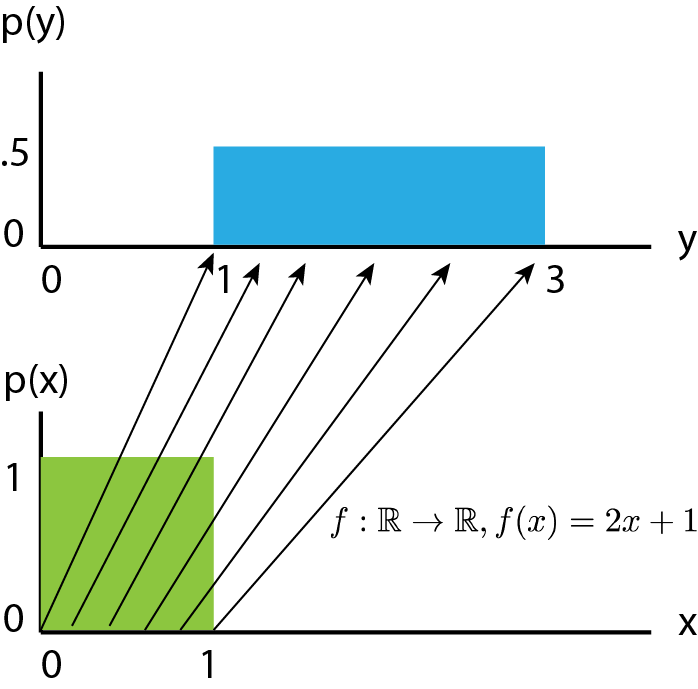
\includegraphics[width=\textwidth]{figures/NF_density_shift.png}
			\caption{Shifting density}
			\label{fig:NF_density_shift}
		\end{subfigure}
		\caption{Outline of how a normalizing flow works}
		\label{fig:NF}
	\end{figure} 
	\item Mathematically, we can define a normalizing flow by:
	\begin{equation*}
		\begin{split}
			x & = z_k = f_k \circ f_{k-1} \circ ... \circ f_1 (z_0) \to z_i = f_i(z_{i-1})\\
			p(z_i) & = p(z_{i-1}) \cdot \left|\det \frac{f_{i}^{-1}}{z_i}\right| \implies p(x) = p(z_0) \cdot \prod_{i=1}^{K} \left|\det \frac{f_{i}^{-1}}{z_i}\right|\\
			\log p(x) & = \log p(z_0) - \sum_{i=1}^{K} \log \left|\det \frac{f_{i}}{z_i}\right|
		\end{split}
	\end{equation*}
	\item Requirements: $f$ must be invertible (dimensions of $x$ and $z$ equal), and the Jacobian must be easy to compute (i.e. triangular)
\end{itemize}